\documentclass[a4paper,11pt,twoside,pdftex]{article}

% Caption package for formating figure and label captions
\usepackage[font=bf,format=hang,labelsep=colon,justification=justified,singlelinecheck=false,compatibility=false]{caption}

% Misc packages
\usepackage{ifthen} % for conditional expressions
\usepackage{float} % for floating tables and graphics
\usepackage{setspace} % for defining spacing between lines
\usepackage{cmap} % allow searching in pdf documents
\usepackage{tabulary} % better tables
\usepackage{comment} % block comments

\usepackage[usenames, dvipsnames]{color} % Highlighting text for editing

% hyperref for HTML links within pdf 
% EXAMPLE: \href{http://www.niwa.co.nz}{NIWA}
\usepackage[bookmarks=true,bookmarksopen=false,bookmarksnumbered=true,
            pdfpagelayout=TwoPageRight,
            pdftitle={CASAL2 Contributors Manual}, 
            pdfauthor={C. Marsh} %authors
            pdfsubject={Casal2, Contributors manual},
            pdftex]{hyperref}
\hypersetup{
  breaklinks=true,      % allow line breaks in URLs
  colorlinks=true,      % use colour to define links
  linkcolor=black,      % colour of internal links
  citecolor=black,      % colour of links to bibliography
  filecolor=black,      % colour of file links
  urlcolor=darkgray     % colour of external links
}
\pdfadjustspacing=1

% Use AMS Maths 
\usepackage[fleqn]{amsmath}
\newcommand\AddVspace{\\[0 pt]} % artificial method of adding vertical space within equations

% Package for including and pretty printing of external config files and program code
\usepackage{listings} 
\lstset{ %
basicstyle=\ttfamily\footnotesize,
breaklines=true,
columns=fullflexible,
showspaces=false,               % show spaces adding particular underscores
showstringspaces=false,         % underline spaces within strings
showtabs=false,                 % show tabs within strings adding particular underscores
tabsize=2,			            % sets default tabsize to 2 spaces
breakatwhitespace=false,	    % sets if automatic breaks should only happen at whitespace
escapeinside={\%*}{*)}          % if you want to add a comment within your code
}

% highlighting package for editing
\usepackage{color,soul}

% Allow colour for HTML links
\usepackage{color}
\definecolor{darkgray}{gray}{0.20}
\definecolor{lightgray}{gray}{0.95}

% Geometery for A4 layout like MS-Word defaults
\usepackage[left=2.54cm,top=2.54cm,bottom=3.17cm,right=3.17cm]{geometry}

% Natlib to better cite references (round brackets, commas between refs, and sorted)
\usepackage[round,comma,sort]{natbib}

% Making the index
\usepackage{makeidx}
\makeindex

% Graphics (no postscript files.. just use jpeg, png, etc)
\usepackage[dvips]{graphicx}
% Changes fonts to Times, Helvetica, Courier
\usepackage{pslatex} 

% Section header fonts
\usepackage{sectsty}
\allsectionsfont{\sffamily\large} % Normal sized arial style section headings
% Add a dot after section headings
\makeatletter
 \def\@seccntformat#1{\csname the#1\endcsname.\quad}
 \renewcommand\paragraph{\@startsection{paragraph}{4}{\z@}%
             {-2.5ex\@plus -1ex \@minus -.25ex}%
             {1.25ex \@plus .25ex}%
             {\normalfont\normalsize\bfseries}}
\makeatother

\setcounter{secnumdepth}{4} % how many sectioning levels to assign numbers to
\setcounter{tocdepth}{4}    % how many sectioning levels to show in ToC

% Page style
\usepackage{fancyhdr}
\pagestyle{fancy}
\fancyhead{}
\fancyfoot{}
\headheight 15pt
\renewcommand{\headrulewidth}{0pt} % rule line under header
\renewcommand{\footrulewidth}{0pt}
\setlength{\parindent}{0pt} % No indentation at start of paragraph
\setlength{\baselineskip}{1ex plus 0.2ex minus 0.1ex}
\setlength{\parskip}{1.1ex} % Gap between paragraphs
\raggedbottom % prefer space at the bottom of page
						
% Make equation numbers be section number then equation number
\makeatletter
\@addtoreset{equation}{section}
\@addtoreset{figure}{section}
\@addtoreset{table}{section}
\def\thefigure{\thesection.\@arabic\c@figure}
\def\thetable{\thesection.\@arabic\c@table}
\def\theequation{\thesection.\@arabic\c@equation}
\makeatother

%% stop figures from going onto a page by themselves 
\renewcommand{\topfraction}{0.85}
\renewcommand{\textfraction}{0.1}
\renewcommand{\floatpagefraction}{0.75}

%% make list gaps small
\usepackage{tweaklist} % (a local style) for tweaking spacing between list elements
\renewcommand{\enumhook}{\setlength{\topsep}{0.5ex}%
  \setlength{\itemsep}{0.1ex}}
\renewcommand{\itemhook}{\setlength{\topsep}{0.5ex}%
  \setlength{\itemsep}{0.1ex}}
%\renewcommand{\descripthook}{\setlength{\topsep}{0.5ex}%
%  \setlength{\itemsep}{0.1ex}}
  
% Minimise hyphen use
\hyphenpenalty=5000
\tolerance=1000

% Compact titles
%\usepackage[small,compact]{titlesec} 

% New commands to define macros and other aids to text and layout
\newcommand{\config}{input configuration file}
\newcommand{\command}[1] {\texttt{@#1}}
\newcommand{\subcommand}[1] {\texttt{#1}}
\newcommand{\commandsub}[2] {\command{#1}\subcommand{.#2}}
\newcommand{\commandlabsub}[2] {\command{#1\texttt{[label]}}\subcommand{.#2}}
\newcommand{\argument}[1] {\texttt{#1}}
\newcommand{\commandsubarg}[3] {\command{#1}\subcommand{.#2}\argument{=#3}}
\newcommand{\commandlabsubarg}[3] {\command{#1\texttt{[label]}}\subcommand{.#2}\argument{=#3}}

\newcommand{\commentline}{\#}
\newcommand{\commentstart}{\{}
\newcommand{\commentend}{\}}

\newcommand{\textlow}[1]{\raisebox{-.4ex}{\scriptsize #1}}

% command shortcuts:
\newcommand{\Rzero}{\emph{R}$_0$}
\newcommand{\Bzero}{\emph{B}$_0$}
\newcommand{\R}{\textbf{R}}
\newcommand{\SSBoff}{$SSB_{\text{offset}}$}

%quick index:
\newcommand{\I}[1]{#1\index{#1}}

% New commands to template syntax definitions: copied from SPM, setup needs defining
% Define a command without a label
\newcommand{\defCom}[2]{\texttt{\textbf{@#1}\index{Command ! #1}} \hspace{0.5cm} {#2}}
% Define a command with a label
\newcommand{\defComLab}[2]{\texttt{\textbf{@#1}\ \emph{label}\index{Command ! #1}} \hspace{0.5cm} {#2}}
% Define a subcommand
\newcommand{\defSub}[2]{\texttt{#1} \hspace{0.5cm} #2 \\*}% Define a command with an argument
\newcommand{\defComArg}[3]{\texttt{\textbf{@#1}\ \emph{#2}\index{Command ! #1}} \hspace{0.5cm} {#3}}
% Define a Command\index{Command} argument
\newcommand{\defArg}[2]{\emph{\texttt{#1}} \hspace{0.5cm} #2 \\*}

% Generic definition for subcommand syntax: copied from SPM, setup needs defining
\newcommand{\defText}[2]{\hangindent=0.3cm \small{#1\ #2}\normalsize \\*}
% Define subcommand syntax for Type / Default / Condition / Value / Note / Example / Lower Bound / Upper Bound
\newcommand{\defType}[1]{\defText{Type:}{#1}}
\newcommand{\defDefault}[1]{\defText{Default:}{#1}}
\newcommand{\defCondition}[1]{\defText{Condition:}{#1}}
\newcommand{\defValue}[1]{\defText{Value:}{#1}}
\newcommand{\defNote}[1]{\defText{Note:}{#1}}
\newcommand{\defExample}[1]{\defText{Example:}{#1}}
\newcommand{\defLowerBound}[1]{\defText{Lower Bound:}{#1}}
\newcommand{\defUpperBound}[1]{\defText{Upper Bound:}{#1}}
\newcommand{\defAllowedValues}[1]{\defText{Allowed Values:}{#1}}

% Input CASAL2 version definitions
%% WARNING: THIS FILE IS AUTOMATICALLY GENERATED BY doBuild documentation. DO NOT EDIT THIS FILE
\newcommand{\SourceControlRevisionDoc}{e4f654c21617d51489766ed65896df048a708392}
\newcommand{\SourceControlDateDoc}{2017-10-22}
\newcommand{\SourceControlYearDoc}{2017}
\newcommand{\SourceControlMonthDoc}{October}
\newcommand{\SourceControlTimeDoc}{19:24:30}
\newcommand{\SourceControlShortVersionDoc}{2017-10-22 (rev. e4f654c2)}
\newcommand{\SourceControlVersionDoc}{2017-10-22 19:24:30 UTC (rev. e4f654c2)}

%\newcommand{\DocYear}{\SourceControlYearDoc}
%\newcommand{\DocMonth}{\SourceControlMonthDoc}
%\newcommand{\DocDate}{\SourceControlMonthDoc\ \SourceControlYearDoc}
%\newcommand{\DocVer}{\SourceControlDateDoc}

%New commands to automate document dates, manual titles, document reference, etc.
%\newcommand{\VER}{v\SourceControlDateDoc} % CASAL2 program version
\newcommand{\CNAME}{\textsc{Casal2}} 
\newcommand{\cname}{\texttt{casal2}} % casal2 binary name
\newcommand{\authors}{C. Marsh and S. Rasmussen}
\newcommand{\email}{casal2@niwa.co.nz}
\newcommand{\github}{\url{https://github.com/NIWAFisheriesModelling/CASAL2}}
\newcommand{\authorlink}{\href{mailto:"CASAL2 Development Team"<casal2@niwa.co.nz>?subject=CASAL2:}{authors}} 
%hyper ref for email
\newcommand{\Organisation}{National Institute of Water \& Atmospheric Research Ltd.} %NIWA
%\newcommand{\ManualRef}{\authors\ (\DocYear). \CNAME\ User Manual, \VER. \Organisation\ \emph{NIWA Technical Report 139}. \ref{TotPages} p.} % full document reference

% Define \clearemptydoublepage so-as to have truly blank pages between sections
\let\origdoublepage\cleardoublepage
\newcommand{\clearemptydoublepage}{%
  \clearpage
  {\pagestyle{empty}\origdoublepage}%
}
%% Commands for the license section taken from http://www.gnu.org/licenses/lgpl-3.0.tex
\renewcommand{\labelenumii}{\alph{enumii})}
\renewcommand{\labelenumiii}{\arabic{enumiii})}

% Load package to count the number of pages in document
% For getting number of pages in document (NOT the last page number printed), use \ref{TotPages}
% Load this last to ensure its macros are not overwritten
\usepackage{totpages} 

\makeatother

%Begin the document
\begin{document} 
\hbadness=10000 % to deal with underfull hbox warnings
\sloppy % use sloppy paras


% Title page
\pdfbookmark[1]{CASAL2 Contributors Manual}{title}
\pagenumbering{alph} % alpha not used, but used to remove warnings when page 1 is re-defined below

\begin{titlepage}
  \thispagestyle{empty} % no header/footer/page number on this page
	\begin{center}

		\vspace{1cm}
		\begin{figure}[htp]
			%\begin{left}
			 
\includegraphics[height=2.5cm]{Figures/CASAL2.png}
			%\end{left}
		\end{figure}

		\vspace*{2.5cm}
		\Huge \CNAME\ Contributors Manual \\

		\vspace{2.0cm}
		\huge \authors \\ %Document authors

		%~\vfill
%		\Large NIWA Technical Report 139 \\%Document Date
%		\Large ISSN 1174-2631 \\%Document Date
%		\Large \DocYear \\%Document Date

%		\vspace{1.0cm}
%		\CNAME\ User Manual (modified \DocVer) for use with \cname\texttt{\_\VER}
	
	\end{center}
\end{titlepage}


% Citation page
\fancyfoot[C]{\thepage}
\pagenumbering{roman}

%~\vfill

%\begin{center}
%Citation: \ManualRef    
%\end{center}

% Table of contents
%\clearemptydoublepage{}
\pdfbookmark[1]{Contents}{contents}

\begin{spacing}{0.8} % Reduce space between lines in contents list
\tableofcontents
\end{spacing}

% Table of figures
%\clearemptydoublepage{}
%\pdfbookmark[1]{List of figures}{figures}
%\begin{spacing}{0.8} % Reduce space between lines in contents list
%\renewcommand\listfigurename{List of figures}
%\listoffigures
%\end{spacing}

% Table of tables
%\clearemptydoublepage{}
%\pdfbookmark[1]{List of tables}{tables}
%\begin{spacing}{0.8} % Reduce space between lines in contents list
%\renewcommand\listtablename{List of tables}
%\listoftables
%\end{spacing}

% Document body
\clearemptydoublepage{}
\renewcommand{\headrulewidth}{0.2pt}
\fancyhead[RO]{\slshape \nouppercase \rightmark} % Section headings at top of page (header, odd pages)
\fancyhead[LE]{\slshape \nouppercase \leftmark}  % Section headings at top of page (header, even pages)
\pagenumbering{arabic} % Page numbers a arabic numerals

%\include{equations}

\section{Introduction}\label{sec:introduction}

This document is an introductory help guide for \CNAME, a generalised age-structured population dynamic modelling package. \CNAME\ is run through the command prompt/terminal where it reads text files (configuration files) which defines the model. \CNAME\ then prints output to a screen or a file or errors out gracefully. This short document is aimed at users who are new to \CNAME. \CNAME\ is primarily used on fish populations, but is no means specific to fish population dynamics. \CNAME's predecessor is the primary tool used in assessing New Zealand's tier one stocks, it is also the standard tool used by CCAMLR for modelling Antarctic toothfish. 
\\\\
\CNAME\ is very generalised, highly flexible, and therefore can be a bit daunting at first sight. It has a large number of run modes, settings, and user defined population dynamics choices that can be turned on and off, depending on circumstances such as, population life history and available data. While there is no requirement for a user to see or understand the underlying code base, it has been written so that it is well tested. Great effort has been put into developing a code base that can be easily interpreted by even novice programmers.
\\\\
\CNAME\ is open source, and is covered under the GNU GPL 2.0 licence. See the terms and conditions in the \CNAME\ Technical User Manual \citep{CASAL2}, or type \texttt{casal2 -l} into the command prompt. There is also supplementary information that may be useful to access when getting familiar with \CNAME. \CNAME\ has a comprehensive user manual \citep{CASAL2} which should be consulted for detail on any model component. \CNAME\ also has a contributors guide to help users add any functionality they wish to tackle any problem, the modular structure of the code base can make adding new processes, observations and likelihoods a breeze. If you have any questions, please contact the \CNAME\ development team at \email, even though this is unsupported software we are keen to help with any advancement.
\\\\
The remaining content of this chapter describes requirements and details about how to run, cite, licensing and contact info for \CNAME. If you are new to population modelling then section~\ref{sec:data_requirements} describes the types of data that you would need to run a \CNAME\ model. This seemed like a logical start to the document as getting \CNAME\ as you want to know if you have the data before you write the model, unless you are using \CNAME\ as an operating model for simulating data. 
The remaining content of the document goes over how you run \CNAME, the syntax of the configuration files that \CNAME\ uses as inputs, and finally we run through an example.
\\\\
\subsection{Version\label{sec:version}}

\CNAME\ can differ between version, especially as issues are fixed or new features added. The \CNAME\ version number is suffixed with a date/time stamp (\texttt{yyyy-mm-dd}), giving the revision control system UTC date for the most recent modification of the underlying software source code. User manual updates will usually be issued for each minor version or date release of \CNAME.

\subsection{Citing the \CNAME\ Getting Started Guide}
A suitable reference for this document is: 

\ManualRef\index{Citation}\index{Citing \CNAME}
 
\subsection{\I{Software license}\index{GNU GPL v2 licence}}
\
This program and the accompanying materials are made available under the terms of the licence \href{http://www.gnu.org/licenses/old-licenses/gpl-2.0.en.html}{GNU GPL v2} which accompanies this software.

Copyright \copyright 2015-\SourceControlYearDoc, \href{http://www.niwa.co.nz}{\Organisation}. All rights reserved.

\subsection{\I{System requirements}}

\CNAME\ is available for most IBM compatible machines running 64-bit \I{Linux} and \I{Microsoft Windows} operating systems.

Several of \CNAME's tasks are highly computer intensive and a fast processor is recommended. Depending on the model implemented, some of \CNAME's tasks can take a considerable amount of time (minutes to hours), and in extreme cases can even take several days to undertake an MCMC estimate. 

The program itself requires only a few megabytes of hard-disk space but output files can consume large amounts of disk space. Depending on number and type of user output requests, the output could range from a few hundred kilobytes to several hundred megabytes. When estimating model fits, several hundred megabytes of RAM may be required, depending on the spatial size of the model, number of categories, and complexity of processes and observations. For extremely large models, several gigabytes of RAM may occasionally be required. 

\subsection{\I{Necessary files}}

For both 64-bit Linux and Microsoft Windows, only the executable file \texttt{casal2} or \texttt{casal2.exe} is required to run \CNAME with non-auto differentiable minimisers. If you wish to use the auto differentiable minimisers the \texttt{.dll} for windows and \texttt{.so} for Linux must be in the same folder as the executable \CNAME\ files or in your system path. No other software is required. We do not compile a version for 32-bit operating systems. 

\CNAME\ offers an \R\ library for post-processing of model output, so we suggest users download software such as \href{http://www.r-project.org}{\R}\ \citep{R} to assist in the post processing of \CNAME\ output (see the \CNAME User Manual Chapter 17 (Post=Processing) for more detail on the \R\ package).

\subsection{Getting help\index{Getting help}\index{User assistance}\index{Notifying errors}}

\CNAME\ is distributed as unsupported software, however we would appreciate being notified of any problems or errors in \CNAME. See the \CNAME\ User manual \citep{CASAL2} for the recommended template for reporting issues.



\section{Creating a local repository\label{sec:local_repo}}

This section will cover the following points

\begin{enumerate}
	\item Registering a github username
	\item Download git software
	\item Fork the master repository
\end{enumerate}

\subsection{Git Username and Profile}

The first step is to create a username and profile on github (if you do not already have one). Creating a username and profile on github is free and easy to do. 

Go to \url{https://www,github.com} to register a username and set up a profile if you do not already have one. See the help at github for more information. Once you have set up a github account you need download the git software that you use to ``communicate" with repositories (places where the software source code is stored) on github.

\subsection{Git Software}

You will need to acquire a git client in order to clone a copy of the source code and link this to the repository.

\CNAME\ also requires a command line version of git in order to compile. The \CNAME\ build environment requires git in order to evaluate the version of the code used at compile time to include into the executable and manual when being built. 

One package that allows this on a Microsoft Windows platform is tortoisegit (see \url{https://tortoisegit.org/download}) to pull, push and commit changes to git repositories. However there are many other clients that could be used to achieve the same functionality.

\subsection{Cloning a repository}

The publicly available \CNAME\ code is in the master repository. Only the \CNAME\ Development Team have permission to add, delete, or change code in the master repository. Other contributors can either add, delete, or change code either by forking the master repository' or by maintaining a local version of the repository. Forking a copy on github can be done at \url{https://github.com/NIWAFisheriesModelling/CASAL2} by selecting the fork button in the top right of the page circled in Figure~\ref{fig:fork}

\begin{figure}[!ht]
	\centering
	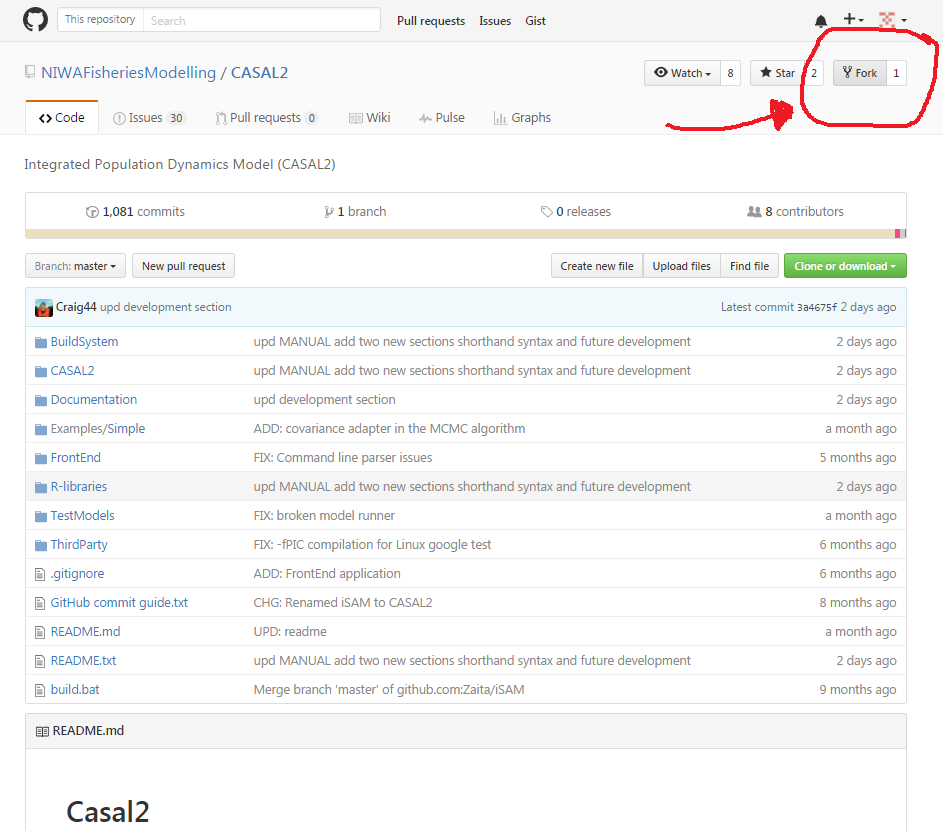
\includegraphics[scale=0.6]{Figures/Fork_button.png}
	\caption{Creating a forked repository}\label{fig:fork}
\end{figure}
\pagebreak

This will create a copy of the \CNAME\ repository under your profile at the point of the fork. To check that you have successfully forked the repository, go to your git profile and you should see a \CNAME\ repository under your repositories, shown in Figure~\ref{fig:fork_success},

\begin{figure}[!ht]
	\centering
	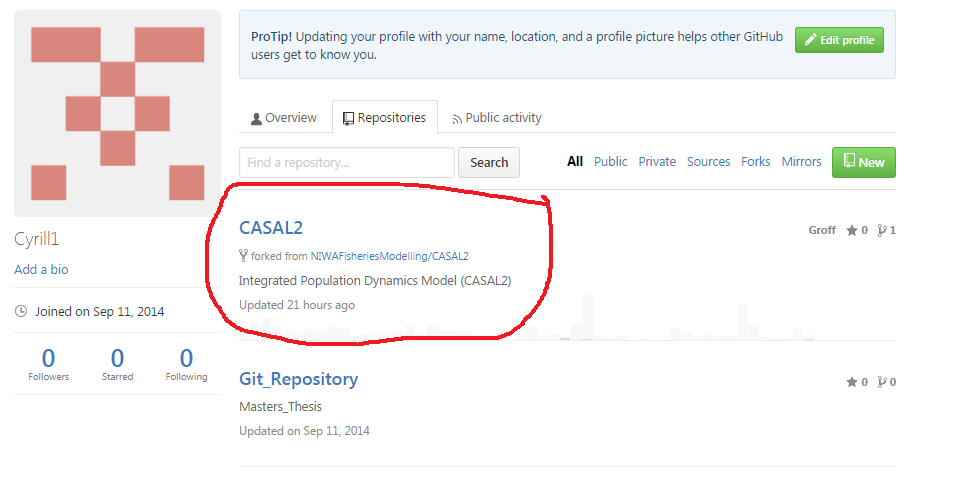
\includegraphics[scale=0.6]{Figures/fork_success.png}
	\caption{Fork success}\label{fig:fork_success}
\end{figure}

An important point is that the forked repository will not automatically keep up to date with the master repository. So if the master changes, you will want to keep your forked repository up to date. This can easily be done and is explained in the next section.




\section{Maintaining and contributing to a forked repository\label{sec:maintain_repo}}

This section covers the following details

\begin{enumerate}
	\item Checking the status of the forked repository compared to the master repository
	\item Updating forked repository
	\item Making changes to your forked repository
\end{enumerate}

\subsection{Checking the status of the forked repository}

The status of the forked repository as compared to the master repository can be seen on github ()see Figure~\ref{fig:fork_status})

\begin{figure}[!ht]
	\centering
	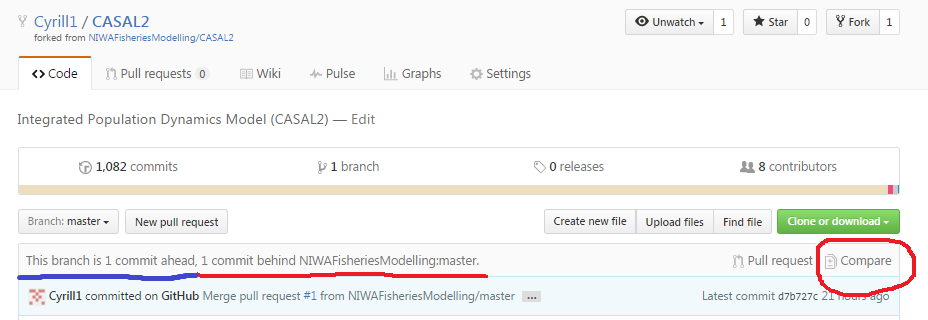
\includegraphics[scale=0.6]{Figures/fork_status.png}
	\caption{Fork status}\label{fig:fork_status}
\end{figure}

This line underlined in blue indicates how many commits have occurred on the forked repo since forking the repo or updating the forked repo. The line underlined in red indicates the commits that have occurred to the master since you forked the repo or last updated it. In the above example, we have made one commit to our forked repo (indicated by the blue) and the forked version is one commit behind the master (indicated by the red). 



\subsection{Updating the forked repository to incorporate changes committed to the master}

To update your forked repository to be the same as the master, click the `compare' button (circled in red on the right of Figure~\ref{fig:fork_status}). This will bring up a page that will tell you of the changes that have occurred to the master repository. 
\clearpage
\begin{figure}[!ht]
	\centering
	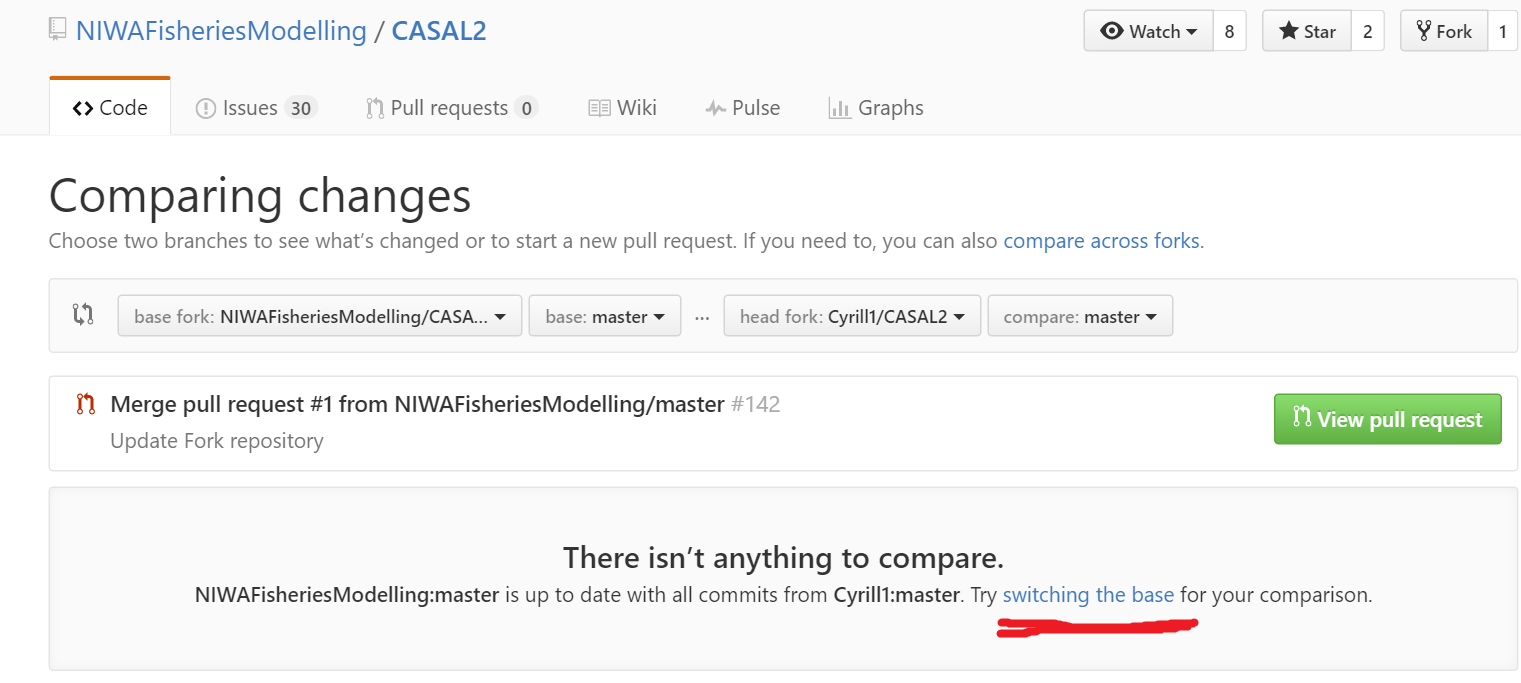
\includegraphics[scale=0.6]{Figures/Compare_fork3.png}
	\caption{}\label{fig:fork_compare1}
\end{figure}

If the following figure appears (Figure~\ref{fig:fork_compare1}) telling you "there isn't anything to compare" click on the \texttt{switching the base} underlined in red.
\raggedbottom
\begin{figure}[!ht]
	\centering
	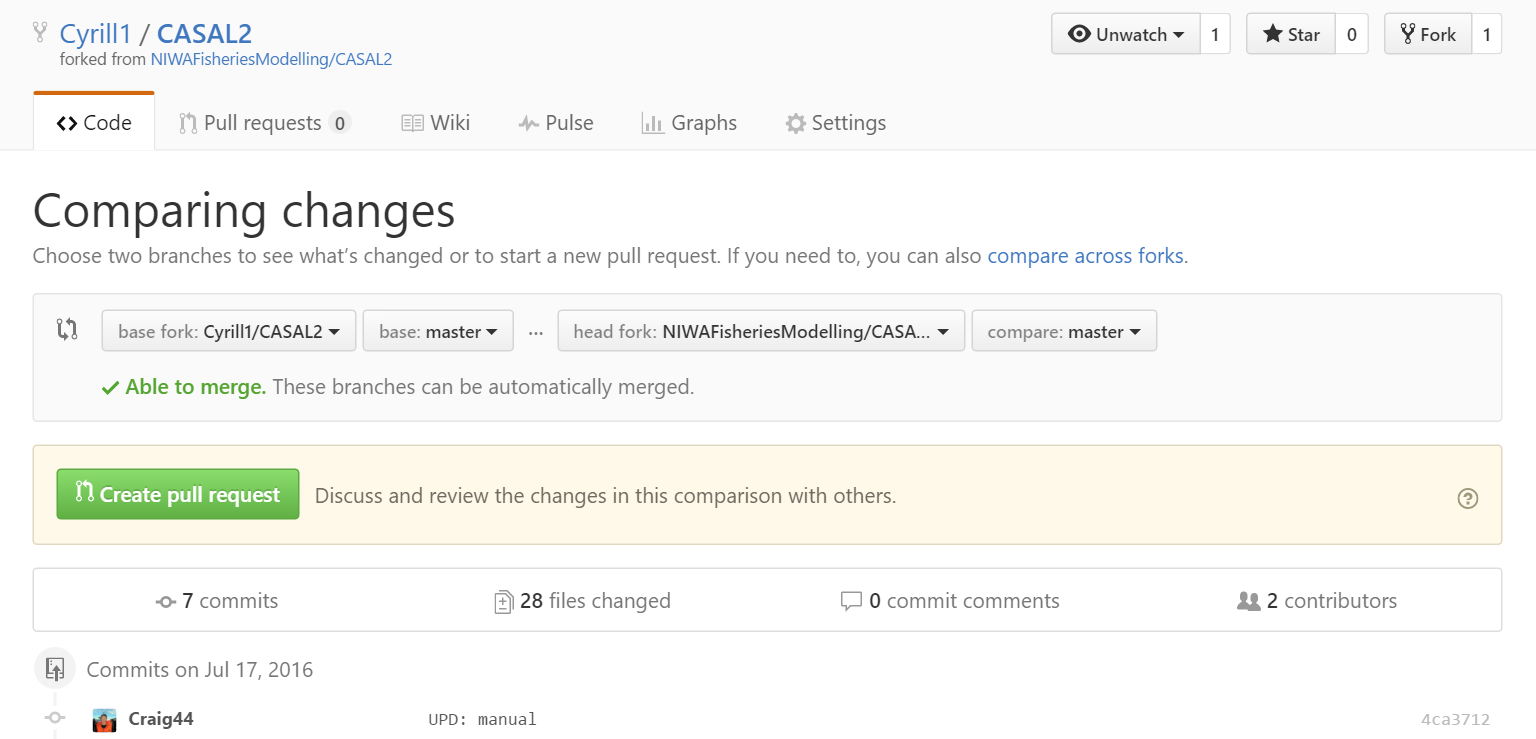
\includegraphics[scale=0.6]{Figures/Compare_fork4.png}
	\caption{}\label{fig:fork_compare2}
\end{figure}

You can see that there are 7 commits and 28 files changed on the master that we want to merge into our forked repo. You can see that there is now a "create pull request" and a green message saying "Able to merge". This indicates you will be able to update your forked repo with ease. Click on the "create pull request" button. This will open a git pull request (Figure~\ref{fig:fork_compare3}) we suggest adding a nice title for the merge like "Updating Craig's Forked Repository" 
\clearpage
\begin{figure}[!ht]
	\centering
	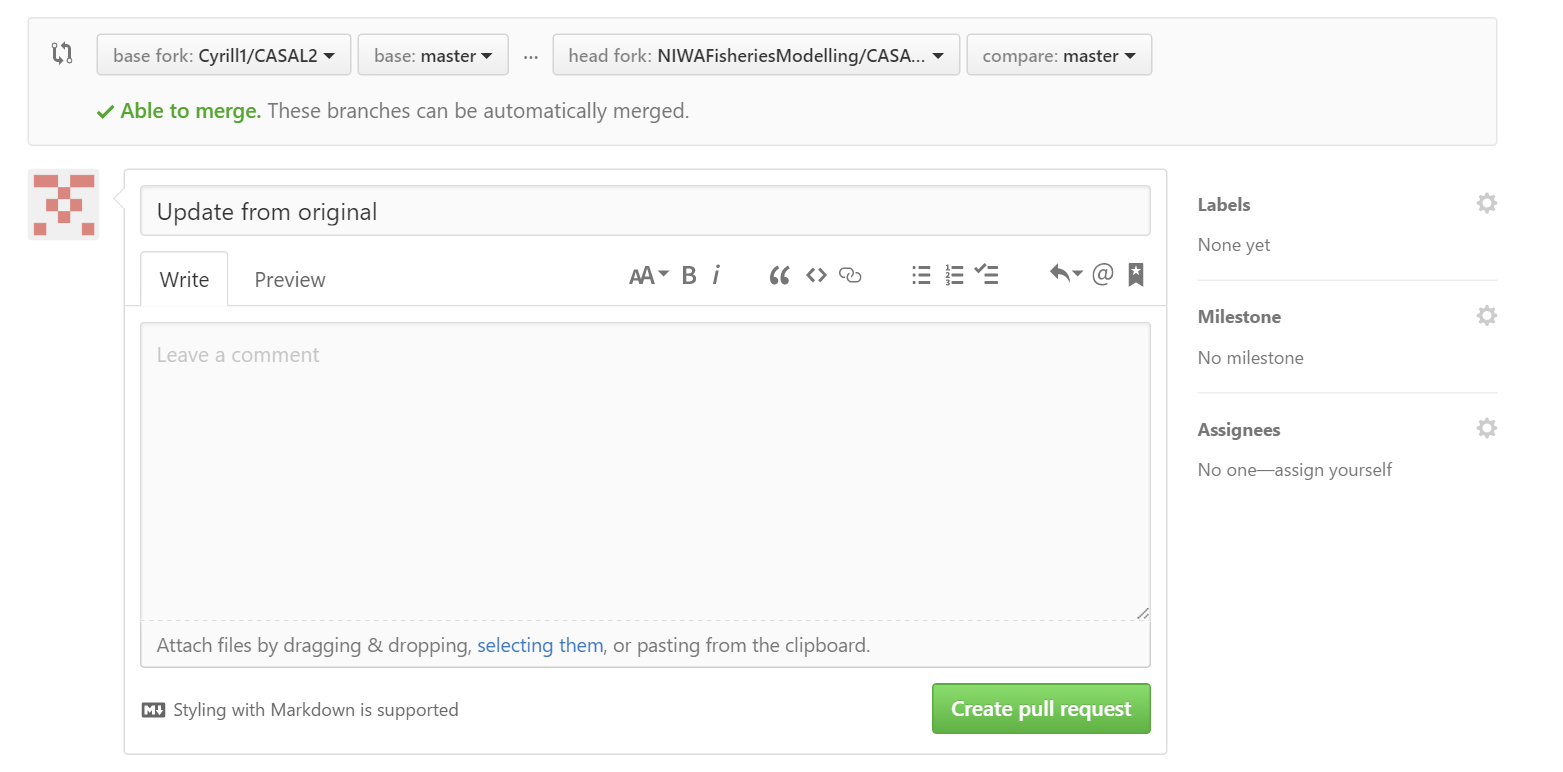
\includegraphics[scale=0.6]{Figures/Compare_fork5.png}
	\caption{}\label{fig:fork_compare3}
\end{figure}

Once you write a reasonable title and click create pull request if there are no conflicts, you can merge teh changes from the master into your forked repo by clicking "merge pull request" form Figure~\ref{fig:fork_compare4}.

\begin{figure}[!ht]
	\centering
	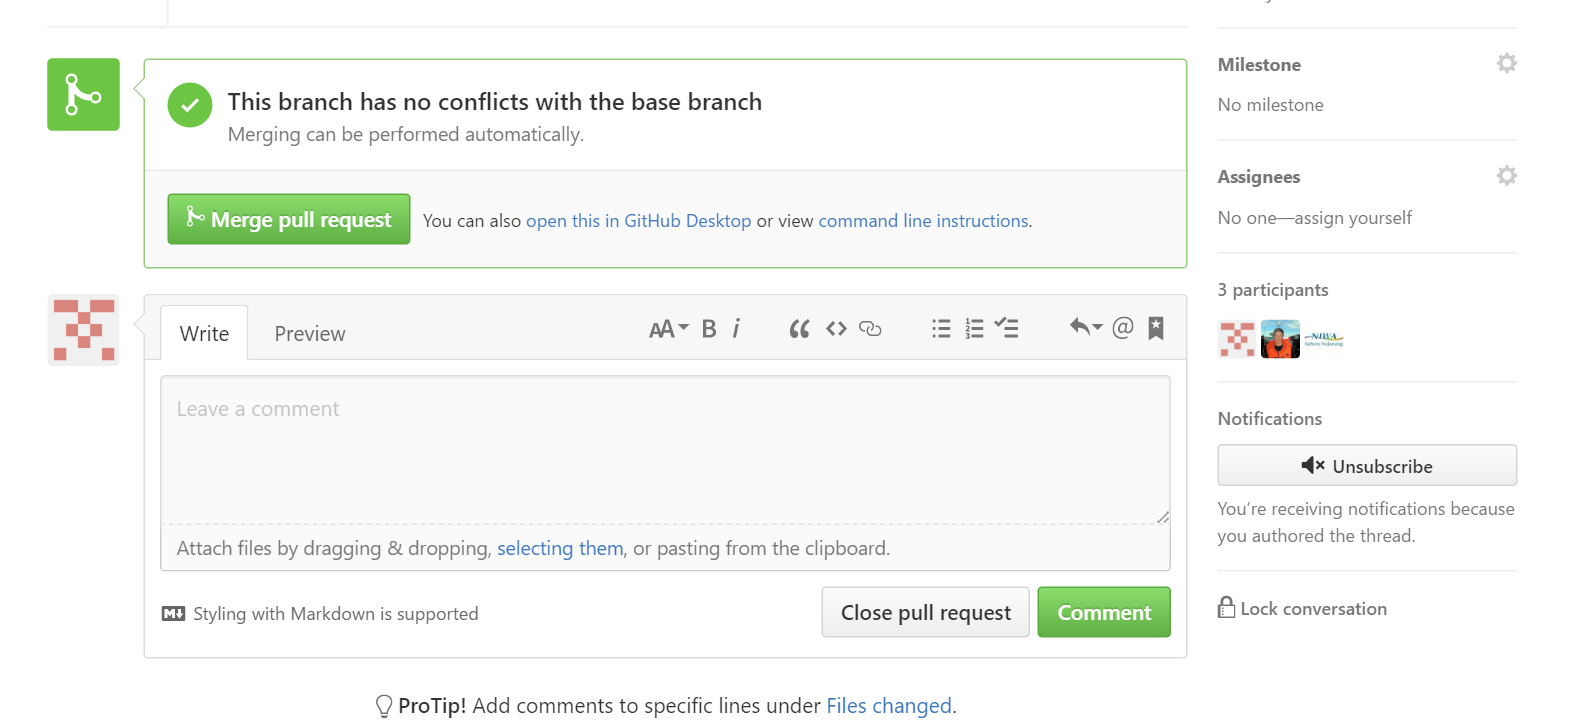
\includegraphics[scale=0.6]{Figures/Compare_fork6.png}
	\caption{}\label{fig:fork_compare4}
\end{figure}
\clearpage
Once you have clicked that you will be told that the merge was a success as shown in Figure~\ref{fig:fork_compare5}.
\begin{figure}[!ht]
	\centering
	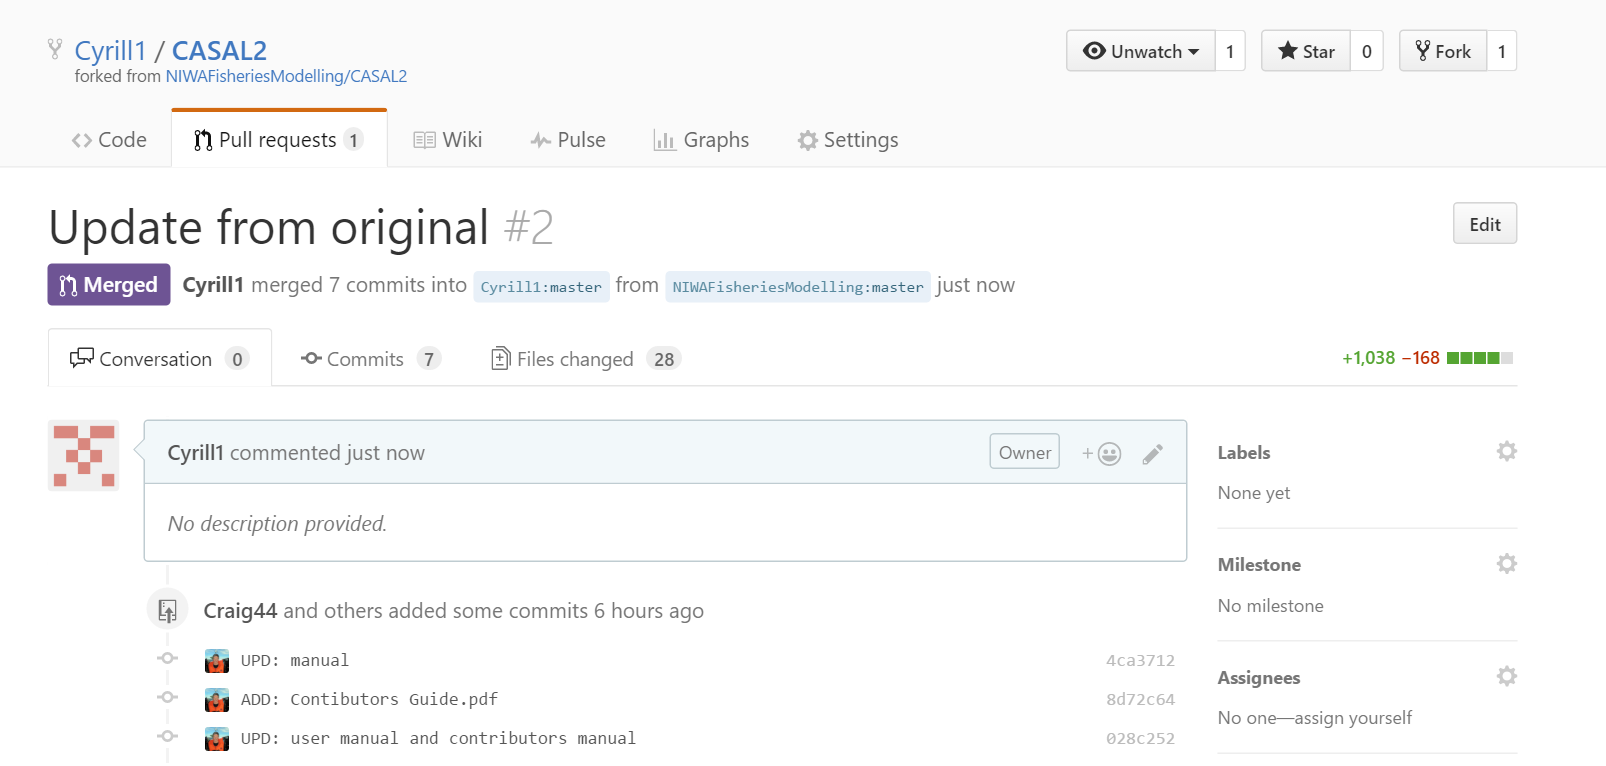
\includegraphics[scale=0.6]{Figures/Compare_fork7.png}
	\caption{}\label{fig:fork_compare5}
\end{figure}

Now you have successfully updated your remote forked repository. To incorporate these changes into your local repository on your computer you just need to do a pull and the code changes should be incorporated in your next build.


\section{Setting up \CNAME\ BuildSystem\label{sec:build_environment}}

This section descibes how to set up the environment on your local machine that will allow you to build and compile \CNAME\. The buld enviroment can be on either Microsoft Windows or Linux systems. At present the \CNAME\ build system supports Microsoft Windows 7+ and Linux (with GCC/G++ 4.9.0+). Apple OSX or other platforms are not currently supported.

\subsection{Overview}

The build system is made up of a collection of python scripts that do various tasks. These are located in \path{CASAL2/BuildSystem/buildtools/classes/}. Each python script has it’s own set of functionality and undertakes one set of actions. 

The top level of the build system can be found at \path{CASAL2/BuildSystem/}. In this directory you can run \texttt{doBuild.bat help} from the command line in Microsoft Windows systems or \texttt{./doBuild.sh help} from a terminal in Linux systems.

The build system will take one or two parameters depending on what style of build you'd like to achieve. These commands allow the building of various stand-alone binaries, shared libraries, and the documentation. Note that you will need additional software installed on your system in order to build \CNAME . These requirements are described later.

A summary of all of the doBuild arguments can be found using the command \texttt{doBuild help} in the BuildSystem directory.

The current arguments to doBuild are: 

\begin{itemize}
  \item \texttt{debug}:  Build standalone debug executable
  \item \texttt{release}: Build standalone release executable
  \item \texttt{test}: Build standalone unit tests executable
  \item \texttt{documentation}: Build the user manual
  \item \texttt{thirdparty}: Build all required third party libraries
  \item \texttt{thirdpartylean}: Build minimal third party libraries
  \item \texttt{clean}: Remove any previous debug/release build information
  \item \texttt{cleanall}: Remove all previous build information
  \item \texttt{archive}: Build a zipped archive of the application. The application is built using shared libraries so a single casal2 executable is created. 
  \item \texttt{check}: Do a check of the build system
  \item \texttt{modelrunner}: Run the test suite of models
  \item \texttt{installer}: Build an installer package
  \item \texttt{deb}: Create Linux .deb installer
  \item \texttt{library}: Build shared library for use by front end application
  \item \texttt{frontend}: Build single CASAL2 executable with all minimisers and unit tests
\end{itemize}

Valid Build Parameters: (thirdparty only)
\begin{itemize}
  \item \texttt{<libary name>}: Target third party library to build or rebuild
\end{itemize}

Valid Build parameters: (debug/release only)
\begin{itemize}
  \item \texttt{betadiff}: Use BetaDiff auto-differentiation (from CASAL)
  \item \texttt{cppad}: Use CppAD auto-differentiation
  \item \texttt{adolc}: Use ADOLC auto-differentiation in compiled executable
\end{itemize}

Valid Build parameters: (library only)
\begin{itemize}
  \item \texttt{adolc}: Build ADOLC auto-differentiation library
  \item \texttt{betadiff}: Build BetaDiff auto-differentiation library (from CASAL)
  \item \texttt{cppad}: Build CppAD auto-differentiation library
  \item \texttt{test}: Build Unit Tests library
  \item \texttt{release}: Build release library
\end{itemize}

The outputs from the build system commands will be placed in subfolders of \path{CASAL2/BuildSystem/bin/<operating system>/<build_type>}

For example:

\path{CASAL2/BuildSystem/windows/debug}

\path{CASAL2/BuildSystem/windows/library_release}

\path{CASAL2/BuildSystem/windows/thirdparty/}

\path{CASAL2/BuildSystem/linux/library_release}

\subsection{Building on Windows}

\subsubsection{Prerequisite Software}

The building of \CNAME\ requires additional build tools and software, including git version control, GCC compiler, LaTex compiler, and an Windows package builder. \CNAME\ requires specific implementations and versions in order to build. 

\textbf{C++ and Fortran Compiler}

Source: tdm-gcc (MingW64) from \url{http://www.tdm-gcc.tdragon.net/}.

\CNAME\ is designed to compile under GCC on Microsoft Windows and Linux  platforms. While it may be possible to build the package using different compilers, the \CNAME\ Development Team does provide any assistance or recommendations. We recommend using 64-bit TDM-GCC version 5.1.0. Ensure you have the gfortran and openmp options installed as a part of TDM-GCC otherwise \CNAME will not compile. \textbf{Note}: A common error that can be made is having a different GCC compiler in your path when attempting to compile. For example, rtools includes a version of the GCC compiler. We recommend removing these from your path prior to compiling.

\textbf{GIT Version Control}

Source: Command line GIT from \url{https://www.git-scm.com/downloads}.

\CNAME\ automatically adds a version number based on the GIT version of the latest commit to its repository. The command line version of GIT is used  to generate a version number for the compiled binaries, R libraries, and the manuals. 

\textbf{MiKTeX Latex Processor}

Source: Portable version from url{http://www.miktex.org/portable}. 

The main user documentation for \CNAME\ is a PDF manual generated from LaTeX. The LaTeX syntax sections of the documentation are generated, in part, directly from the code. In order to regenerate the user documentation, you will need the MiKTeX LaTeX compiler.

\textbf{7}
The BuildSystem calls 7zip.exe to unzip files in the build system it is advised to have this in the path.

\textbf{Inno Setup Installer Builder (optional)}

Source: Inno Setup 5 from \url{http://www.jrsoftware.org/isdl.php}

If you wish to build a Microsoft Windowes compatible Installer for \CNAME\ then you will need the Inno Setup 5 application installed on the machine. The installation path must be \path{C:\Program Files (x86)\Inno Setup 5\} in order for the build scipts to fins and use it.

\subsubsection{Pre-Build Requirements}

Prior to building \CNAME\ you will need to ensure you have both G++ and GIT in your path. You can check both of these by typing:

\texttt{g++ --version}

\texttt{git --version}

This also allows you to check that there are no alternative versions of a GCC compiler that may confuse the \CNAME\ build. 

It’s worth checking to ensure GFortran has been installed with the G++ compiler by typing:

\texttt{gfortran --version}

If you wish to build the documentation bibtex will also need to be in the path:

\texttt{bibtex -version}

\subsubsection{Building \CNAME}

The build process is relatively straightforward. You can run \texttt{doBuild check} to see if your build environment is ready.

\begin{enumerate}
  \item Get a copy (clone) of the forked code on your local machine, mentioned in Section~\ref{sec:local_repo}: 
  \item Navigate to the BuildSystem folder in \path{CASAL2/BuildSystem}
  \item You need to build the third party libraries with:
  \begin{itemize}
    \item \texttt{doBuild thirdparty}
  \end{itemize}
  \item You need to build the binary you want to use:
  \begin{itemize}
    \item \texttt{doBuild release}
  \end{itemize}	
  \item You can build the documentation if you want:
  \begin{itemize}
    \item \texttt{doBuild documentation}
  \end{itemize}		
\end{enumerate}

\subsection{Building on Linux}

This guide has been written against a fresh install of Ubuntu 15.10. With Ubuntu we use apt-get to install new packages. You’ll need to be familiar with the package manager for your distribution to correctly install the required prerequisite software.

\subsubsection{Prerequisite Software}

\textbf{Compiler G++}

Ubuntu 15.10 comes with G++ 15.10, gfortran is not installed though so we can install it with: \texttt{sudo apt-get install gfortran}.

\textbf{GIT Version Control}

Git isn't installed by default but we can install it with \texttt{sudo apt-get install git}

\CNAME\ automatically adds a version number based on the GIT version of the latest commit to its repository. The command line version of GIT is used  to generate a version number for the compiled binaries, R libraries, and the manuals. 

\textbf{CMake}

CMake is required to build multiple third-party libraries and the main code base. You can do this with \texttt{sudo apt-get install cmake}

\textbf{Python2 Modules}

There are a couple of Python2 modules that are required to build \CNAME. These can be installed with \texttt{sudo apt-get install python-dateutil}

You may also need to install \textbf{datetime}, re and \textbf{distutils}. \textbf{Texlive} Latex Processor. No supported latex processors are installed with Ubuntu by default. You can install a suitable latex process with:

\texttt{sudo apt-get install texlive-binaries}
\texttt{sudo apt-get install texlive-latex-base}
\texttt{sudo apt-get install texlive-latex-recommended}
\texttt{sudo apt-get install texlive-latex-extra}

Alternatively you can install the complete package:
\texttt{sudo apt-get install texlive-full}

\subsubsection{Building \CNAME}

The build process is relatively straighforward. You can run \texttt{./doBuild.sh check} to see if your build environment is ready.

\begin{enumerate}
	\item Get a copy (clone) of the forked code on your local machine, mentioned in Section~\ref{sec:local_repo}: 
	\item Navigate to the BuildSystem folder in \path{CASAL2/BuildSystem}
	\item You need to build the third party libraries with:
	\begin{itemize}
	    \item \texttt{./doBuild.sh thirdparty}
	\end{itemize}
	\item You need to build the binary you want to use:
	\begin{itemize}
		\item \texttt{./doBuild.sh release}
	\end{itemize}	
	\item You can build the documentation if you want:
	\begin{itemize}
		\item \texttt{./doBuild.sh documentation}
	\end{itemize}		
\end{enumerate}

\subsection{Troubleshooting}

\subsubsection{Third-party Libraries}

It’s possible there will be build errors or issues building the third-party libraries. If you encounter an error then it’s worth checking the log files. Each third-party build system stores a log of everything it’s doing. The files will be named

\begin{itemize}
	\item casal2\_unzip.log
	\item casal2\_configure.log
	\item casal2\_make.log
	\item casal2\_build.log
	\item \dots etc,.
\end{itemize}

Some of the third-party libraries require very specialised environments for compiling under GCC on Windows. These libraries are packaged with MSYS (MinGW Linux style shell system). The log files for these will be found in \path{ThirdParty/<library name>/msys/1.0/<library name>/}

e.g: \path{ThirdParty/adolc/msys/1.0/adolc/ADOL-C-2.5.2/casal2_make.log}

\subsubsection{Main Code Base}

If the unmodified code base does not compile, the most likely cause is an issue with the third-party libraries not being built. Ensure they have been built correctly. As they are outside the control of the Development Team, problems can arise that may require the developers of the third party libraries to resolve first. Contact the \CNAME\ development team at \texttt{casal2@niwa.co.nz} for help.





\section{\CNAME\ build rules\label{sec:build_rules}}

This section describes the standards and requirements for code to be included within the \CNAME\ code base. 

\subsection{\CNAME\ coding practice and style}\label{subsec:code_practive}

\CNAME\ is written in C++ and follows the Google C++ style guide (see \url{https://google.github.io/styleguide/cppguide.html}). The guide is long and comprehensive, so we don't necessarily recommend that you read or understand all of its content. However, the Development Team would like you to follow the Google style of code layout and structure. Google provides a handy script to parse source code and highlight errors that do not match their coding style.

This means using good indentations for functions and loops, sensible (human readable) variable names but noting the use of the characters `\_' on the end of class variables defined in the .h files. 

\textbf{Annotate} your code. For readability we encourage you to put lots of comments in your code. This helps others read what you intended. 

On top of annotating your code we encourage developers to add descriptive logging statements (print messages) in the code. You will see this in the source code already. The purpose of this is to allow a descriptive summary of the actions being done in the model for debugging purposes and curious users. By using these, it becomes easier to identify issues, errors and creates a transparent model for users.

You can also output the text and equations in these logs that would normally be too detailed for general users to be interested, as this may allow users to verify the exact equations or processes that have been implemented. These are really there for curious users and developers.

There are different levels of logging in \CNAME\ listed below.
\begin{itemize}
	\item LOG\_MEDIUM()  usually reserved for iterative functionality (e.g. estimates during estimation phase)
	\item LOG\_FINE() the level of reporting between an actual report and a fine scale detail that end users are not interested in (Developers)
	\item LOG\_FINEST() Minor details
	\item LOG\_TRACE() put at the beginning of every function
\end{itemize}

To run \CNAME\ in log mode piping out any LOG\_FINEST and coarser logs (LOG\_MEDIUM and LOG\_FINE) you can use the following command,

\texttt{casal2 -r --loglevel finest > MyReports.csl2 2> log.out}

This will output all the logged information to \texttt{log.out}.

\subsection{Unit tests}

One of the key focusses in the \CNAME\ development is an emphasis on software integrity --- this is to help ensure that the results from implemented models are consistent and error free. As part of this, we use unit tests to check the individual components of the code base, as well as tests that run entire models in order to validate that the outputs are what we expect them to be.

\CNAME\ uses:
\begin{itemize}
	\item Google testing framework
	\item Google mocking framework
\end{itemize}

When adding unit tests, they need to be developed and tested outside of \CNAME\  first, for example in \R\ or another program like \CNAME\ e.g. CASAL or Stock Synthesis. This gives confidence that the test does not contain a calcualtion or other error. 

An example of how to add a unit test for a process is shown in Section~\ref{sec:example}

\subsection{Reporting (Optional)}

Currently \CNAME\ has reports that are \R\ compatible, i.e., all output reports produced by \CNAME\ can be read into \R\ using the standard  \textbf{CASAL2} \R\ package. If you create a new report or modify an old one, you most follow the standard so that the report is \R\ compatible.

All reports must start with,
\texttt{*label (type)}
and end with,
\texttt{*end}

Depending on what type of information you wish to report, will depend on the syntax you need to use. For example

\paragraph*{$\{$d$\}$ (Dataframe)}
Report a dataframe
{\small{\begin{verbatim}
*estimates (estimate_value)
values {d}
process[Recruitment_BOP].r0 process[Recruitment_ENLD].r0 
2e+006 8e+006
*end
\end{verbatim}}}

\paragraph*{$\{$m$\}$ (Matrix)}
Report a matrix
{\small{\begin{verbatim}
*covar (covariance_matrix)
Covariance_Matrix {m}
2.29729e+010 -742.276 -70160.5
-110126 -424507 -81300 
-36283.4 955920 -52736.2 
*end
\end{verbatim}}}

\paragraph*{$\{$L$\}$ (List)}
Report a List
{\small{\begin{verbatim}
*weight_one (partition_mean_weight)
year: 1900
ENLD.EN.notag {L}
mean_weights {L}
0.0476604 0.111575 0.199705
end {L}
age_lengths {L}
12.0314 16.2808 20.0135
end {L}
end {L}
*end
\end{verbatim}}}

\subsection{Update manual}
The syntax sections of the user manual are automatically generated from the source code. This means contributors will need to add or modify the remaining sections of the the user manual to document their changes. This is a requirement of contributed or suggested code changes, and is important for end users to be able to use the new or modified functionality.

\subsection{Builds to pass before merging changes}

Once you have made changes to the code, you must run the following builds before your changes can be considered for includion in the the main code base.

build the unittest version see Section~\ref{sec:build_environment} for how to build unittest depending on {\color{red}your} system.

Run the standard and new unit tests to check that they all pass
\texttt{DoBuild test}

And test that the debug and release of \CNAME\ compile and run.
\texttt{DoBuild debug}

Then run the second phase of unit tests (requires the debug version is built). This runs the tests that comprise of complete model runs
\texttt{DoBuild modelrunner}

Build the archive 
\texttt{DoBuild archive}




\section{Merging changes form a forked repository to a master repository\label{sec:pull_requests}}
This section will cover, how to merge changes from a forked repository to the 'master' repository. This is under the assumptions that the contributor has followed all the rules laid out in Section~\ref{sec:build_rules}.

\end{document}
%End